\documentclass[12pt]{article}
%\documentclass[12pt, fleqn]{article}
\usepackage{mathptmx}
\usepackage{fullpage}
\usepackage{graphicx}
\usepackage{amsmath}
\usepackage{outlines}
\usepackage{listings}
%\usepackage{xcolor}
\usepackage[table]{xcolor}

\usepackage{multirow}
\usepackage{multicol}
\usepackage{booktabs}
\lstset { %
	language=R,
	backgroundcolor=\color{black!5}, % set backgroundcolor
	basicstyle=\footnotesize,% basic font setting
}

%Regression table preamp
\usepackage{pdflscape}
\usepackage{booktabs,caption}
\usepackage[flushleft]{threeparttable}
\usepackage{siunitx} % Formats the units and values
\usepackage{pgfplotstable} % Generates table from .csv
\usepackage{booktabs}

%\documentclass[preprint,floatfix] {revtex4} 
\newcommand{\rvec}{\mathrm {\mathbf {r}}} 
\usepackage{subfigure}
\usepackage{color, soul}


% Setup siunitx:
\sisetup{
	round-mode          = places, % Rounds numbers
	round-precision     = 4, % to 2 places
}

\newcolumntype{M}[1]{>{\centering\arraybackslash}m{#1}}
\newcolumntype{N}{@{}m{0pt}@{}}

\usepackage{float}

\title{Housing and Credit Cycles}
\author{Nam Nguyen}
\date{\today}                                          

\begin{document}
	\maketitle
	
	\begin{outline}[enumerate]
		
		\section{Motivation}
		
		This paper uses a multivariate extension of the model proposed by Morley et al. (2003) and Huang and Kishor (2018)
		
		The novel contribution of this paper is the inclusion of cross transitory components effect as seen in eq(5) \& eq(6). I would like to take advantage of it to explore the dynamics of the relationship between housing prices and house hold credit in the short run.
		
		\section {Model Specification}
		
		\textbf{\textit{Series:}} \\
		-Credit : Credit to non financial sector\\
		-HPI : Housing Price Index
		\begin{align}
		ln \frac{Credit}{GDP} &= y_t = \tau_{yt} + c_{yt}
		\\
		ln HPI &= h_t = \tau_{ht} + c_{ht}
		\end{align}
		\\
		\textbf{\textit{Trends:}}
		
		A random walk drift term $g_t$ is added in the stochastic trend inspired by Clark (1987)
		\begin{align}
		\tau_{yt} &= \tau_{yt-1} + \eta_{yt}, &\eta_{yt} \sim iidN(0,\sigma^2_{\eta y})
		\\
		\tau_{ht} &= \tau_{ht-1} + \eta_{ht}, &\eta_{ht} \sim iidN(0,\sigma^2_{\eta h})	
		\end{align}
		\\
		\textbf{\textit{Cycles:}}
		\begin{align}
		c_{yt} &= \phi^1_{y}c_{yt-1}  
		+ \phi^2_{y}c_{yt-2}  
		+ \phi^x_{y}c_{ht-1} 
		+ \varepsilon_{yt},
		&\varepsilon_{yt} \sim iidN(0,\sigma^2_{\varepsilon y})		   
		\\
		c_{ht} &= \phi^1_{h}c_{ht-1}  
		+ \phi^2_{h}c_{ht-2}
		+ \phi^x_{h}c_{yt-1}  
		+ \varepsilon_{ht},
		&\varepsilon_{ht} \sim iidN(0,\sigma^2_{\varepsilon h})
		\end{align}
		\\
		
		
		\textbf{State-Space Model}
		
		\textit{Transition equation:}
		\begin{align}
		\beta_t = F\beta_{t-1} + \tilde{v}_t
		\end{align}
		
		Where the transitory components are:
		
		\begin{align}
		\begin{bmatrix}
		\tau_{yt}	\\
		c_{yt}		\\
		c_{yt-1}		\\
		\tau_{ht}	\\
		c_{ht}		\\
		c_{ht-1}		
		\end{bmatrix}
		=
		%F matrix
		\begin{bmatrix}
		1	& 0	& 0	& 0	& 0	& 0	\\
		0	& \phi^1_y	& \phi^2_y	& 0	& \phi^x_y	& 0	\\
		0	& 1	& 0	& 0 & 0 & 0  \\
		0	& 0	& 0	& 1	& 0	& 0 \\
		0	& \phi^x_h	& 0	& 0 &\phi^1_h	& \phi^2_h	\\
		0	& 0	& 0	& 0 & 1 & 0
		\end{bmatrix}
		%Bt-1 matrix
		\begin{bmatrix}
		\tau_{yt-1}	\\
		c_{yt-1}		\\
		c_{yt-2}		\\
		\tau_{ht-1}	\\
		c_{ht-1}		\\
		c_{ht-2}		
		\end{bmatrix}
		+
		\begin{bmatrix}
		\eta_{yt}	\\
		\varepsilon_{yt}		\\
		0	\\
		\eta_{ht}	\\
		\varepsilon_{ht}		\\
		0	
		\end{bmatrix}
		\end{align}
		
		\textit{The covariance matrix for $\tilde{v}_t$, denoted Q, is: }
		\begin{align}
		Q = 
		\begin{bmatrix}
		\sigma^2_{\eta y}	& 0	 &0 & 0	& 0	& 0	\\
		0	& \sigma^2_{\varepsilon y}	& 0	& 0	& \sigma_{\varepsilon y \varepsilon h}	& 0	\\
		0	&	0	& 0 & 0 & 0 & 0	\\
		0	& 0	& 0	& \sigma^2_{\eta h}	& 0	& 0	\\
		0	& \sigma_{\varepsilon y \varepsilon h}	& 0	& 0	& \sigma^2_{\varepsilon h}		& 0	\\
		0	&0	& 0	& 0
		& 0	& 0
		\end{bmatrix}
		\end{align}
		
		\textit{Measurement Equation:}
		\begin{align}
		\tilde{y}_t = A + H\beta_t
		\end{align}
		
		\begin{align*}
		\begin{bmatrix}
		y_t	\\
		h_t
		\end{bmatrix}
		=
		\begin{bmatrix}
		0	\\
		0
		\end{bmatrix}
		+
		\begin{bmatrix}
		1	& 0	& 1	& 0	& 0 & 0 \\
		0	& 0 & 0 & 1 & 0 & 1
		\end{bmatrix}
		\begin{bmatrix}
		\tau_{yt}	\\
		c_{yt}		\\
		c_{yt-1}	\\
		\tau_{ht}	\\
		c_{ht}		\\
		c_{ht-1}
		\end{bmatrix}
		\end{align*}
		\pagebreak
\section{Parameters constraints}

The estimation of the unobserved component model uses a nonlinear log-likelihood function maximization. Estimating this function requires numerical optimization.


I did not put stationary constraints directly on the autoregressive parameters. Since such constraints on a VAR(2) system is complex to setup. However, to achieve feasible stationary transitory measurement, I implement an additional term on the objective function:

\begin{align}
l(\theta) = -w1\sum_{t=1}^{T}ln\lbrack(2\pi)^2|f_{t|t-1}|\rbrack
-w2\sum_{t=1}^{T}\eta'_{t|t-1}f^{-1}_{t|t-1}\eta_{t|t-1}
- w3*\sum_{t=1}^{T}(c_{yt}^2) + w4*\sum_{t=1}^{T}(c_{ht}^2)
\end{align}

The last term in the objective function acts as a penalty against too much transitory deviation from zero. Without this penalty, the trend would be linear or all the movements in the measured series would be matched by transitory movements.

\vspace{5mm} %5mm vertical space

Regarding constraints on covariance matrix, I applied the same constraints as in Morley 2007 to imply for positive definite covariance matrix.


\section{Priors selection}

The priors for autoregressive parameters in matrix F are taken from VAR regression of the HP filter cycle decomposition of the series.

For $\beta_{0|0}$, I set $\tau_{0|0}$ as the value of the first available row of data and omit the first observation from the regression. $c_{0|0}$ are set to be equal to their HP filter counterpart. $var(\tau_{0|0}) =100+50*random$; while other measures of the starting covariance are set to be their unconditional values.

Starting standard deviation and correlation values are randomized within reasonable range.

\clearpage

		\section{Data Description}
		Our quarterly data sample periods include periods from January 1989 to January 2020. Table 1 shows the description of the data used in this paper. The sample periods was chosen based on the nature of the change in regulation of credit and housing market beginning early 1990s. The main source of the data comes from the Bank of International Settlement (BIS). The housing price index is based on base index of 2010 as 100. The credit to household data is measured as percentage of GDP.
		
		\begin{table}[]
			\begin{threeparttable}
				\caption {\label{tab:table1} Descriptive statistics}
				\rowcolors{2}{gray!10}{white} 
				\begin{tabular}{@{}llSSSll@{}}
					\toprule
					Country & Index & \multicolumn{1}{c}{Mean} & \multicolumn{1}{c}{Max} & \multicolumn{1}{c}{Min} & \multicolumn{1}{c}{Frequency} & Periods\\
					\midrule
					UK & $y_t$ & 432.0829 & 459.1071 & 406.7316 & Quarterly & 1989:Q1-2020:Q1\\[2pt] 
					
					& $h_t$ & 464.7302 & 503.8838 & 441.5308 & Quarterly & 1989:Q1-2020:Q1\\[2pt] 
					
					US & $y_t$ & 429.0831 & 456.8506 & 395.8907 & Quarterly & 1989:Q1-2020:Q1\\[2pt] 
					
					& $h_t$ & 434.0478 & 480.1792 & 378.2752 & Quarterly & 1989:Q1-2020:Q1\\[2pt] 
					
					\bottomrule
				\end{tabular}
				\begin{tablenotes}
					\small
					\item $y_t$ is credit to household series, $h_t$ is housing price index series. Both are log transformed. \\
				\end{tablenotes}
			\end{threeparttable}
		\end{table}
	

		\begin{table}[]
			\centering
		\begin{threeparttable}
			\caption {\label{tab:table2} Correlation matrix}
%			\rowcolors{2}{gray!10}{white} 
			\begin{tabular}{@{}llll@{}}
				\toprule
				Country & & $y_t$ & $h_t$ \\
				\midrule
				UK & $y_t$ & 1 &  \\[2pt] 
				
				& $h_t$ & 0.9359935 & 1 \\[2pt] 
				\midrule
				US & $y_t$ & 1 &  \\[2pt] 
				
				& $h_t$ & 0.7046029 & 1 \\[2pt] 
				
				\bottomrule
			\end{tabular}
%			\begin{tablenotes}
%				\small
%				\item $y_t$ is credit to household series, $h_t$ is housing price index series. Both are log transformed. \\
%			\end{tablenotes}
		\end{threeparttable}
	\end{table}

		
		\section{Regression results}
		
		In this following section, I will apply the UC model to data from 2 countries: US and UK.
		
Choosing priors from an estimated VAR(2) regression on HP filtered cycle and trend series. The following likelihood function weights are selected in the manner that they make the series look the most stable. 
		
		The regression tables below show Unobserved component VAR(2) regression results with and without cross-cycle parameters.
		
		\pagebreak
		
%		
%		\begin{landscape}
%			
%			%Regression table
%			% Please add the following required packages to your document preamble:
%			% \usepackage{booktabs}
%			% \usepackage{multirow}
%			\begin{table}[]
%				\caption {\label{tab:table1} United States regression results} 
%				\rowcolors{2}{gray!10}{white}
%				\begin{tabular}{@{}lSSSSSS@{}}
%					\toprule
%					\multirow{2}{*}{Parameters} & \multicolumn{2}{c}{VAR(2)} & \multicolumn{2}{c}{VAR(2) 1st-cross-lag} & \multicolumn{2}{c}{VAR(2) 2-cross-lags} \\
%					& \multicolumn{1}{l}{Estimate}     & \multicolumn{1}{l}{Std. Error}  & \multicolumn{1}{l}{Estimate}            & \multicolumn{1}{l}{Std. Error}         & \multicolumn{1}{c}{Estimate}            & \multicolumn{1}{c}{Std. Error}        \\ \midrule
%					$\phi^1_{y}$                & 1.521670374  & 0.323602024 & 1.890301193         & 0.036315042        & 1.886592178         & 0.00028419        \\
%					$\phi^2_{y}$                & -0.592177551 & 0.282758652 & -0.773199508        & 0.021652307        & -0.8941981          & 0.003233388       \\
%					$\phi^{x1}_{y}$             &              &             & -0.012689515        & 0.001245419        & 0.04280046          & 0.000520376       \\
%					$\phi^{x2}_{y}$             &              &             &                     &                    & -0.040322766        & 0.000876719       \\
%					$\phi^1_{h}$                & 1.803961772  & 0.039406338 & 1.465513594         & 0.064627659        & 1.864726867         & 0.038659834       \\
%					$\phi^2_{h}$                & -0.820986013 & 0.039263457 & -0.736886204        & 0.047825955        & -0.898033258        & 0.039051475       \\
%					$\phi^{x1}_{h}$             &              &             & 2.576890191         & 1.642027848        & 0.089729346         & 0.11453162        \\
%					$\phi^{x2}_{h}$             &              &             &                     &                    & -0.031982418        & 0.113620129       \\
%					$\sigma_{ny}$               & 0.968115538  & 0.064573932 & 0.975833563         & 0.066722551        & 0.858997834         & 0.055437867       \\
%					$\sigma_{ey}$               & 0.136584746  & 0.073940054 & 0.000413197         & 0.008728546        & 0.030583756         & 0.016664357       \\
%					$\sigma_{nh}$               & 0.964325946  & 0.107167236 & 1.271977495         & 0.127987617        & 1.135553581         & 0.106041662       \\
%					$\sigma_{eh}$               & 0.471089742  & 0.079046967 & 0.296047479         & 0.161613716        & 0.363776038         & 0.077466523       \\
%					$\sigma_{eyeh}$             & -0.999391959 & 0.03023235  & -0.881232755        & 0.311836698        & -1                  & 5.19E-07          \\
%					$\sigma_{nynh}$             & 0.464225409  & 0.094391207 &                     &                    &                     &                   \\
%					Log-likelihood value        & -369.9163016 &             & -384.7973521        &                    & -363.3991125        &                   \\ \bottomrule
%				\end{tabular}
%			\end{table}
%			
%		\end{landscape}
%		
%		\pagebreak
		
		
		\pagebreak
		
		\begin{landscape}
			
			%Regression table
			\begin{table}[]
				\begin{threeparttable}
				\caption {\label{tab:table1} United Kingdom regression results}
				\rowcolors{2}{gray!10}{white} 
				\begin{tabular}{@{}lSSSSSS@{}}
					\toprule
					\multirow{1}{*}{Parameters} & \multicolumn{2}{c}{VAR(2)} & \multicolumn{2}{c}{VAR(2) 1-cross-lag} & \multicolumn{2}{c}{VAR(2) 2-cross-lags} \\
					& \multicolumn{1}{l}{Estimate}     & \multicolumn{1}{l}{Std. Error}  & \multicolumn{1}{l}{Estimate}            & \multicolumn{1}{l}{Std. Error}         & \multicolumn{1}{c}{Estimate}            & \multicolumn{1}{l}{Std. Error}        \\ \midrule
$\phi^1_{y}$ & 1.9724669930757 & 0.0234468079641688 & 1.88197173053092 & 0.000523125515915717 & 1.88953015161501 & 0.000183792455813221 \\[2pt] 

$\phi^2_{y}$ & -0.982683577200677 & 0.0263416186406314 & -0.815982512675866 & 0.00223671725855314 & -0.874307021294592 & 0.00255445094151967 \\[2pt] 

$\phi^{x1}_{y}$ &  &  & -0.023989100791422 & 0.000359092103478258 & 0.175607246015124 & 0.000809713546032516 \\[2pt] 

$\phi^{x2}_{y}$ &  &  &  &  & -0.196405159419335 & 0.00345072911067609 \\[2pt] 

$\phi^1_{h}$ & 1.50478963225312 & 0.101880883082685 & 1.57483174602634 & 0.00564601795054225 & 1.57420604076636 & 0.0642716927922472 \\[2pt] 

$\phi^2_{h}$ & -0.560771136941685 & 0.125238824672495 & -0.709427180268352 & 0.00767038778223485 & -0.736359754267049 & 0.0585703755604665 \\[2pt] 

$\phi^{x1}_{h}$ &  &  & 0.378335367631202 & 0.0170754712315724 & 0.721371469046458 & 0.0492006408181797 \\[2pt] 

$\phi^{x2}_{h}$ &  &  &  &  & -0.595881261414649 & 0.0442251354127095 \\[2pt] 

$\sigma_{ny}$ & 0.706260098775181 & 0.0599943989318998 & 0.701703618546321 & 0.0352951761051411 & 0.603955648517265 & 0.0374077642345331 \\[2pt] 

$\sigma_{ey}$ & 0.000426758587731293 & 0.0103570158509057 & 0.11272451354988 & 0.00521152792358025 & 0.0160160963024367 & 0.0062789472885429 \\[2pt] 

$\sigma_{nh}$ & 1.86757774805953 & 0.161705655819894 & 1.64285780217825 & 0.102292598525495 & 1.90382148717739 & 0.111540211251835 \\[2pt] 

$\sigma_{eh}$ & 0.656751391241774 & 0.258262683575022 & 0.63234948433104 & 0.0192668720356221 & 0.12891726400829 & 0.0268555883325836 \\[2pt] 

$\sigma_{eyeh}$ & 0.688777773046045 & 13.1231225529083 & 0.999999986940504 & 7.05800130005596e-06 & 0.999771604778545 & 0.00609274849523753 \\[2pt] 

$\sigma_{nynh}$ & 0.568004544830427 & 0.112515260783059 &  &  &  &  \\[2pt] 

Log-likelihood value & -454.645000317534 &  & -464.079327351476 &  & -456.56846781196 &  \\[2pt] 


										
					\bottomrule
				\end{tabular}
			\begin{tablenotes}
				\small
				\item Weights of likelihood function: w1 = 0.6, w2 = 0.4, w3 = 0.004, w4 = 0.003\\
				$l(\theta) = -w1\sum_{t=1}^{T}ln\lbrack(2\pi)^2|f_{t|t-1}|\rbrack
				-w2\sum_{t=1}^{T}\eta'_{t|t-1}f^{-1}_{t|t-1}\eta_{t|t-1}
				- w3*\sum_{t=1}^{T}(c_{yt}^2) + w4*\sum_{t=1}^{T}(c_{ht}^2)$
			\end{tablenotes}
			\end{threeparttable}
			\end{table}
			
		\end{landscape}
		
		\clearpage
		
		\pagebreak
		
		\begin{landscape}
			
			%Regression table
			\begin{table}[]
				\begin{threeparttable}
					\caption {\label{tab:table1} United States regression results}
					\rowcolors{2}{gray!10}{white} 
					\begin{tabular}{@{}lSSSSSS@{}}
						\toprule
						\multirow{1}{*}{Parameters} & \multicolumn{2}{c}{VAR(2)} & \multicolumn{2}{c}{VAR(2) 1-cross-lag} & \multicolumn{2}{c}{VAR(2) 2-cross-lags} \\
						& \multicolumn{1}{l}{Estimate}     & \multicolumn{1}{l}{Std. Error}  & \multicolumn{1}{l}{Estimate}            & \multicolumn{1}{l}{Std. Error}         & \multicolumn{1}{c}{Estimate}            & \multicolumn{1}{l}{Std. Error}        \\ \midrule
						$\phi^1_{y}$ & 1.84966219148423 & 0.0644676313866302 & 1.3049851733765 & 0.104750302567286 & 1.55023948671664 & 0.0621673748460661 \\[2pt] 

						$\phi^2_{y}$ & -0.891729894865282 & 0.0639404413297913 & -0.509866573496016 & 0.069617976248189 & -0.575429145279164 & 0.0642314985800815 \\[2pt] 

						$\phi^{x1}_{y}$ &  &  & 0.0332424600607159 & 0.00266153911071895 & 0.0141314056256322 & 0.00830698240108732 \\[2pt] 

						$\phi^{x2}_{y}$ &  &  &  &  & 0.00368355628246947 & 0.0113623125942596 \\[2pt] 

						$\phi^1_{h}$ & 1.78470130468539 & 0.0344716924207026 & 2.05291126214826 & 0.0420850279485188 & 1.83380271755234 & 0.0658209041054138 \\[2pt] 

						$\phi^2_{h}$ & -0.803434089401448 & 0.0344748867950664 & -1.24693155894687 & 0.0730767847110221 & -0.935812307687759 & 0.0611374033703922 \\[2pt] 

						$\phi^{x1}_{h}$ &  &  & 1.07952833357358 & 0.291843931365872 & 1.7429079493859 & 0.44060251456779 \\[2pt] 

						$\phi^{x2}_{h}$ &  &  &  &  & -1.65444981264612 & 0.417548360352977 \\[2pt] 

						$\sigma_{ny}$ & 0.479256554775164 & 0.024356073491864 & 0.471764807847753 & 0.0240668275640588 & 0.419468168735488 & 0.0205969049394897 \\[2pt] 

						$\sigma_{ey}$ & 0.0281304866214994 & 0.015423818330929 & 0.0256204974500183 & 0.0136254798281635 & 0.0375254711433971 & 0.0132294877888843 \\[2pt] 

						$\sigma_{nh}$ & 0.454891152005456 & 0.0439608378398243 & 0.474208630734516 & 0.0382694791792356 & 0.493724545052865 & 0.0367094830752408 \\[2pt] 

						$\sigma_{eh}$ & 0.256618222235034 & 0.0323339473241677 & 0.0876133859992021 & 0.075599690650887 & 0.0965865013366302 & 0.0477727959889094 \\[2pt] 

						$\sigma_{eyeh}$ & -0.999999981277929 & 0.00012954480904903 & 0.999999998244551 & 8.59389213308525e-05 & 0.999999999996535 & 2.57431114995605e-06 \\[2pt] 

						$\sigma_{nynh}$ & 0.397394222344986 & 0.0720586265329286 &  &  &  &  \\[2pt] 

						Log-likelihood value & -339.725810225008 &  & -346.91597902411 &  & -332.070599830711 &  \\[2pt] 

												
						\bottomrule
					\end{tabular}
					\begin{tablenotes}
						\small
						\item Weights of likelihood function: w1 = 0.8, w2 = 0.2, w3 = 0.003, w4 = 0.004 \\
						$l(\theta) = -w1\sum_{t=1}^{T}ln\lbrack(2\pi)^2|f_{t|t-1}|\rbrack
						-w2\sum_{t=1}^{T}\eta'_{t|t-1}f^{-1}_{t|t-1}\eta_{t|t-1}
						- w3*\sum_{t=1}^{T}(c_{yt}^2) + w4*\sum_{t=1}^{T}(c_{ht}^2)$
					\end{tablenotes}
				\end{threeparttable}
			\end{table}
			
		\end{landscape}
		
		\clearpage
		
%		Given the regression results from the above table. To avoid the problem of perfect collinearity as shown in US data regression, and also to have a more significant estimate of the cross cycle component; I select the second model - VAR(2) with 1 cross lag in the cycle component as the one to focus on.
		
		Regarding results for the UK, the model selection criteria (likelihood function value) indicates that a simple VAR(2) fit the data the best. However, with the introduction of cross-cycle terms, at a slight cost of lower likelihood value I can better estimate the correlation value of short run credit and house price index ($\sigma_{eyeh}$) at a more significant value. Additionally, the cross-cycle results shows a better 
		
		Regression results for the US are less obvious. This could be attributed by the low correlation between the two series as shown in Table 2 and potentially a identification problem. All of the correlation value of short run credit and house price index ($\sigma_{eyeh}$) in all three models show a multicollinearity problem. The model selection criteria shows that VAR(2) with 2-cross-lag coefficients have the highest likelihood value. 
		
		The novel contribution of this paper is to introduce this parameter $\phi^{xt}_h$ in which it measure the effect of a change in last periods credit transitory component on the current housing price transitory component. In both cross-cycle regressions in the UK and US, I can observe that there is a significant positive effect ($\phi^{x1}_{h}$) of last period credit cycle deviation on current housing cycle component. While the coefficients of transitory housing index deviation on household credit ($\phi^{x1}_{y}$) are much smaller. 
		\\
		
		The following graphs shows the UC forecast series against the actual data series.
		
		\begin{figure}[h!]
			\caption{VAR(2) UK: }	
			\centerline{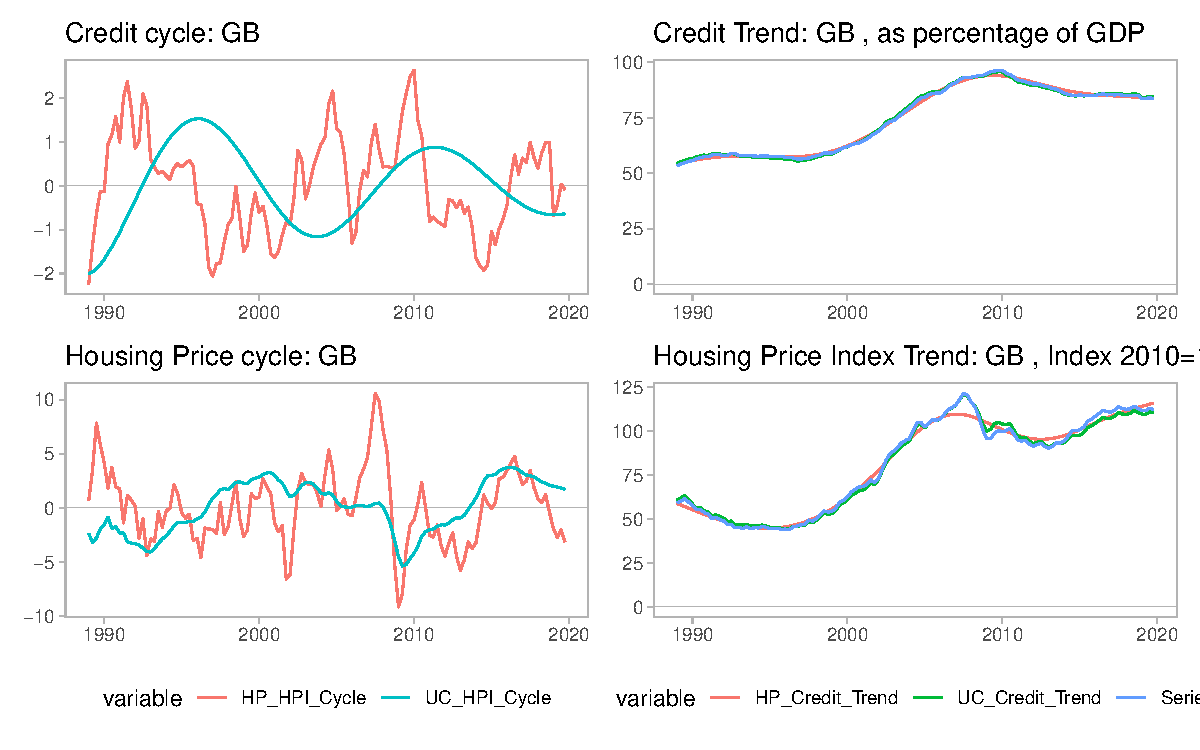
\includegraphics[scale=0.7]{../../Regression/VAR_2/Output/Graphs/HP_Credit_4graphs_GB.pdf}}
		\end{figure}
		
		\clearpage
		
		\begin{figure}[h!]
			\caption{VAR(2) Crosscycle UK: }	
			\centerline{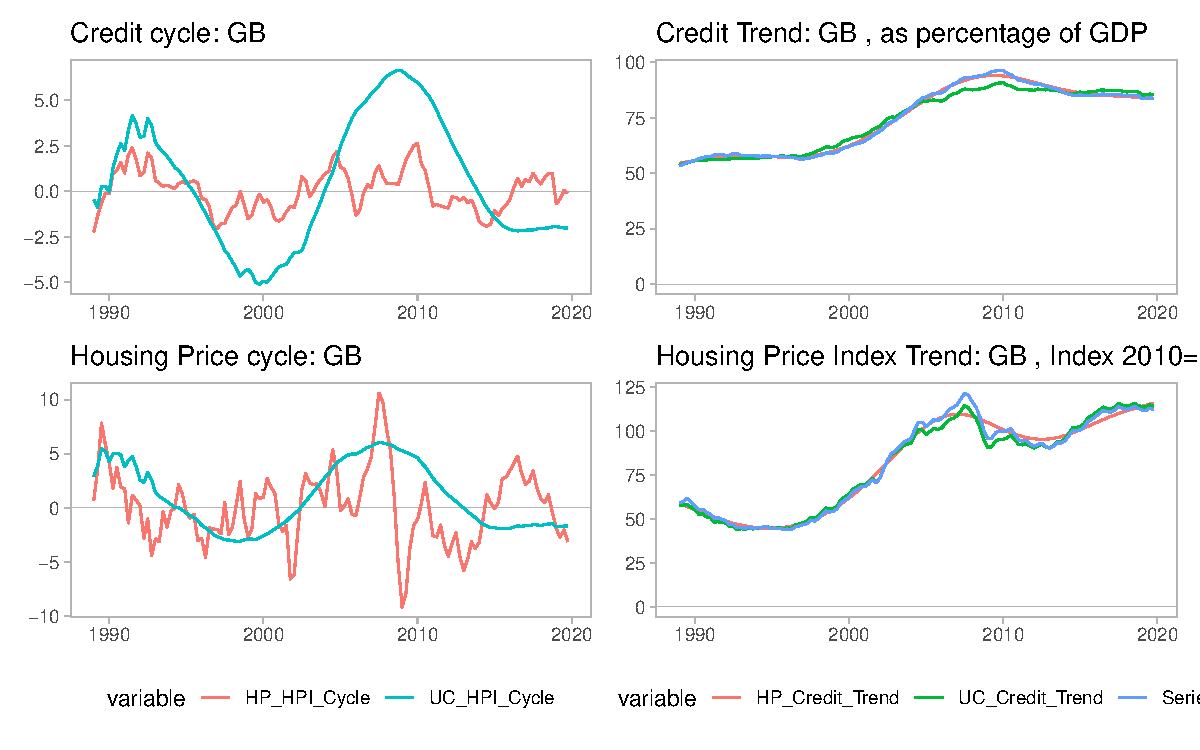
\includegraphics[scale=0.7]{../../Regression/VAR_2_crosscycle/Output/Graphs/HP_Credit_4graphs_GB.pdf}}
		\end{figure}
		
		\clearpage
		
		\begin{figure}[h!]
			\caption{VAR(2) Crosscycle 1st lag only UK: }	
			\centerline{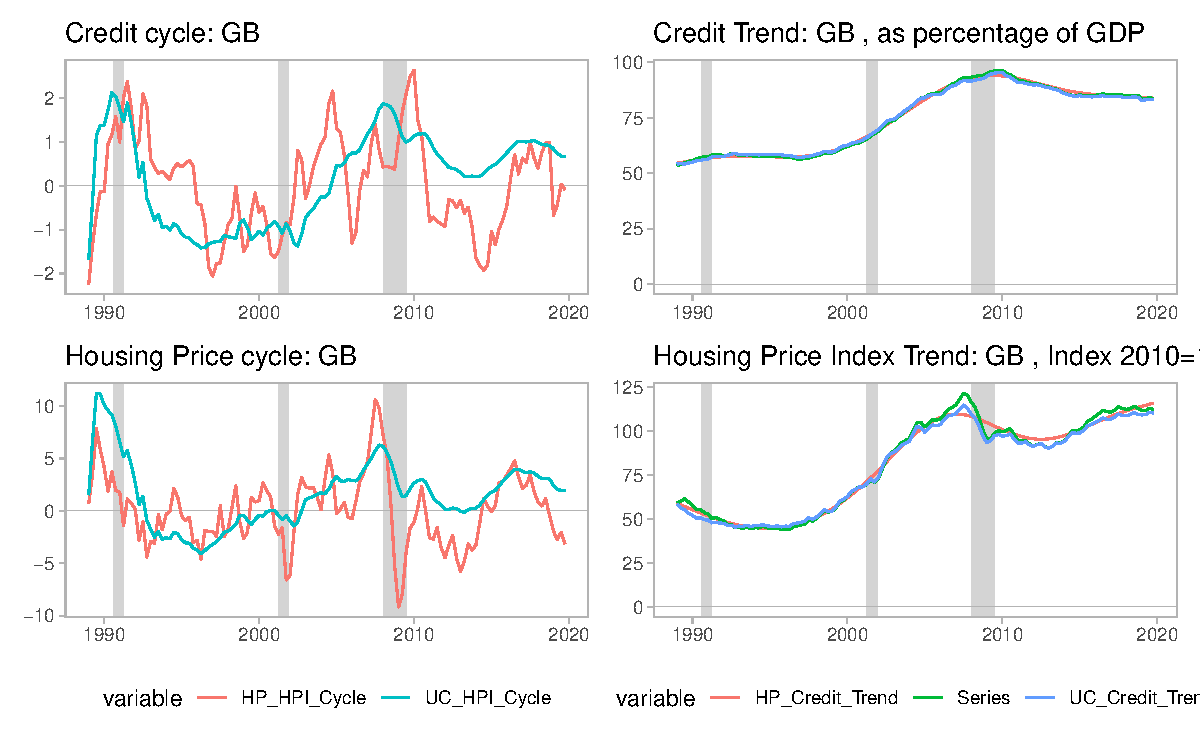
\includegraphics[scale=0.7]{../../Regression/VAR_2_crosscycle_1stlagonly/Output/Graphs/HP_Credit_4graphs_GB.pdf}}
		\end{figure}
		
		\clearpage

		
		\begin{figure}[h!]
			\caption{VAR(2) US: }	
			\centerline{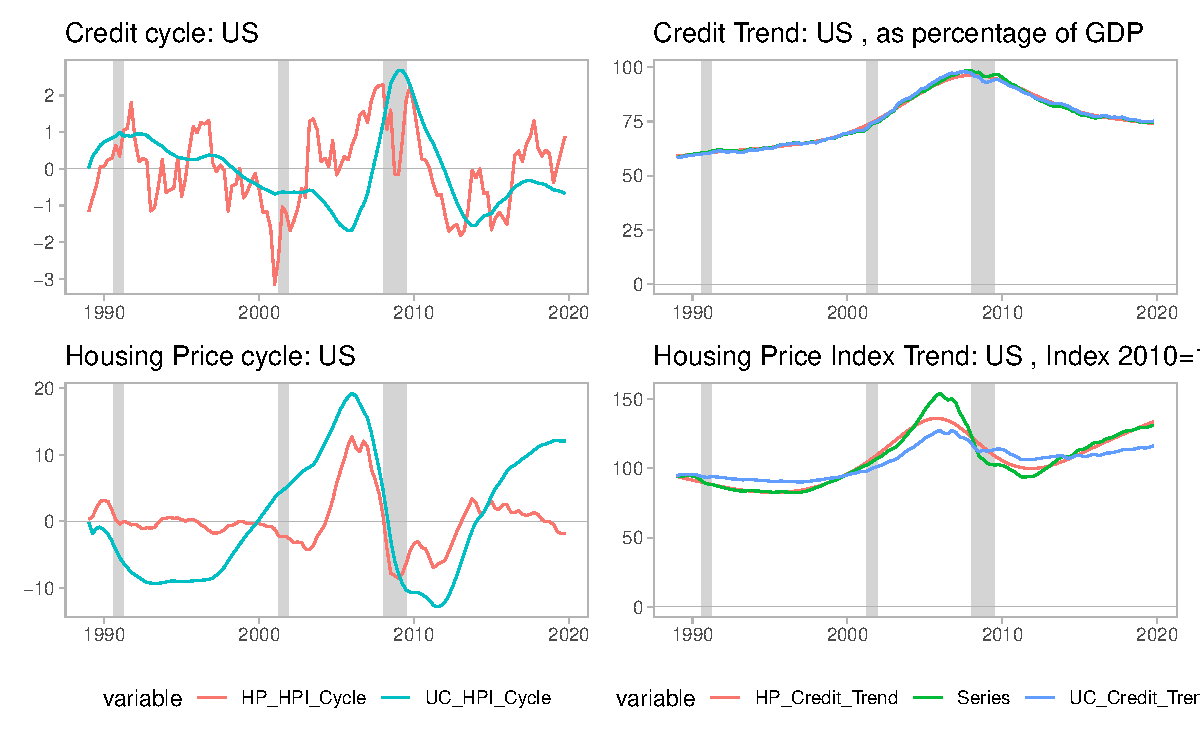
\includegraphics[scale=0.7]{../../Regression/VAR_2/Output/Graphs/HP_Credit_4graphs_US.pdf}}
		\end{figure}
		
		\clearpage
		
		\begin{figure}[h!]
			\caption{VAR(2) Crosscycle US: }	
			\centerline{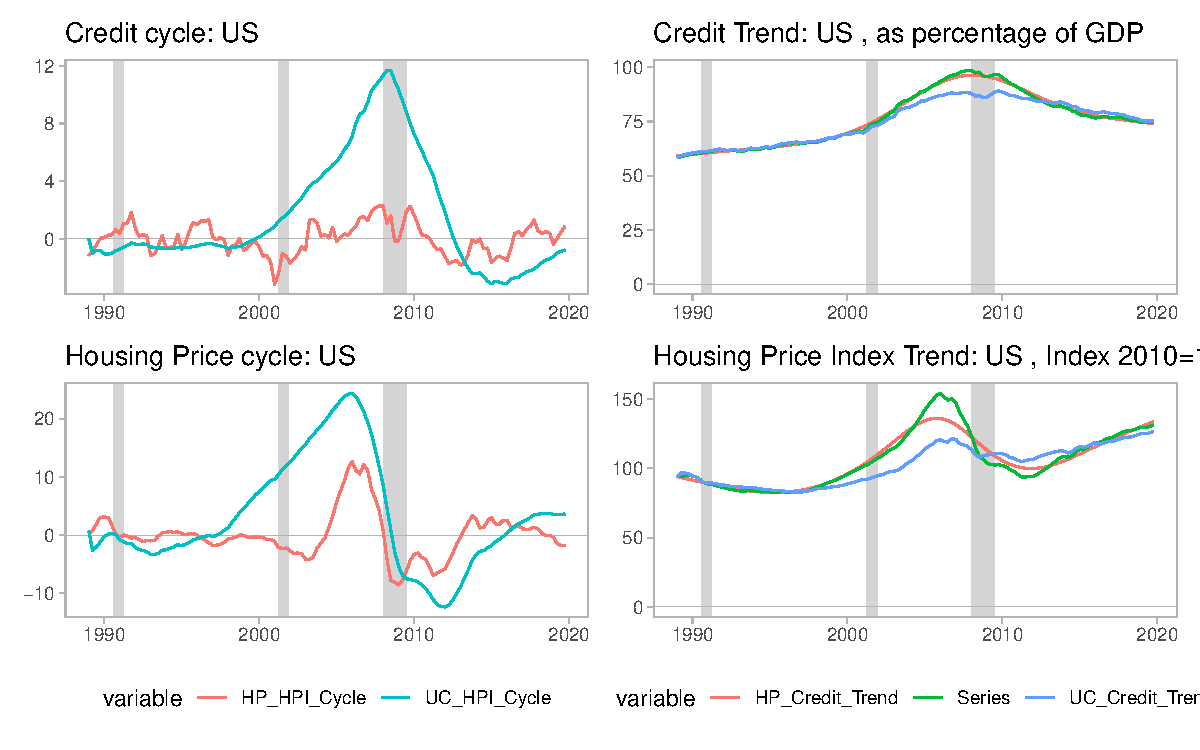
\includegraphics[scale=0.7]{../../Regression/VAR_2_crosscycle/Output/Graphs/HP_Credit_4graphs_US.pdf}}
		\end{figure}
		
		\clearpage
		
		\begin{figure}[h!]
			\caption{VAR(2) Crosscycle 1st lag only US: }	
			\centerline{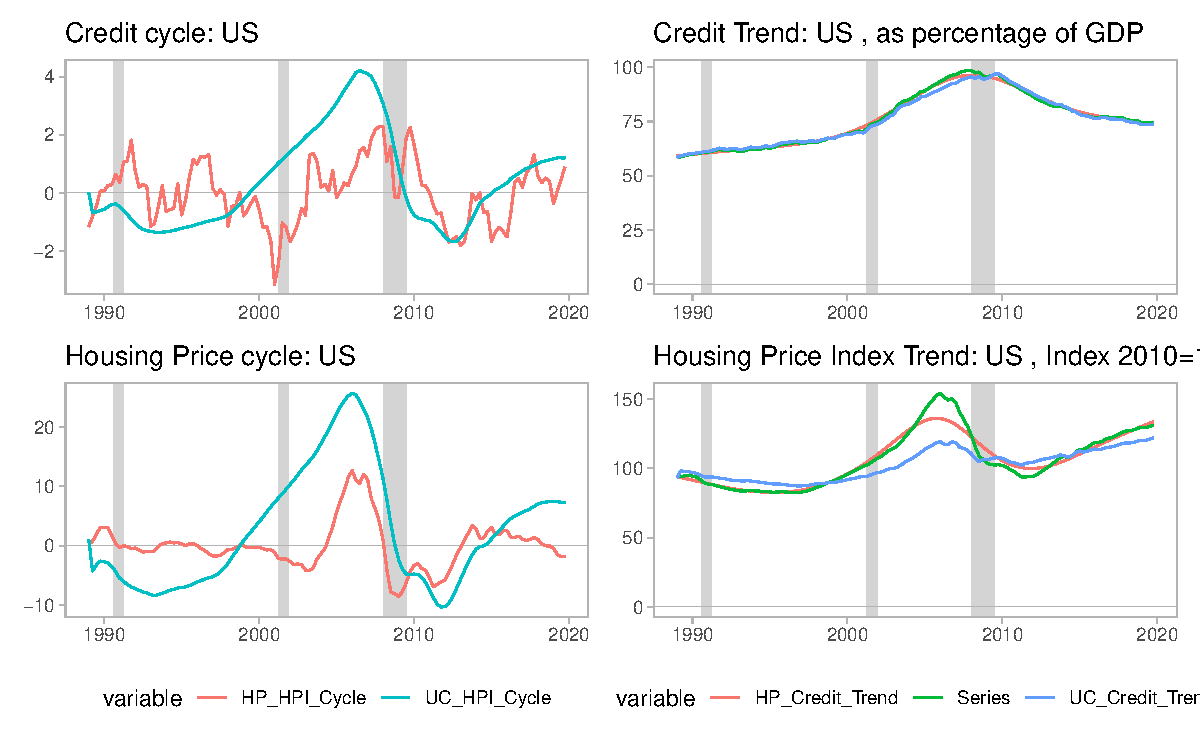
\includegraphics[scale=0.7]{../../Regression/VAR_2_crosscycle_1stlagonly/Output/Graphs/HP_Credit_4graphs_US.pdf}}
		\end{figure}
		
		\clearpage
		
%		\begin{figure}[h!]
%			\caption{VAR(2) cross-cycle 1st lag US: Cycle components}	
%			\centerline{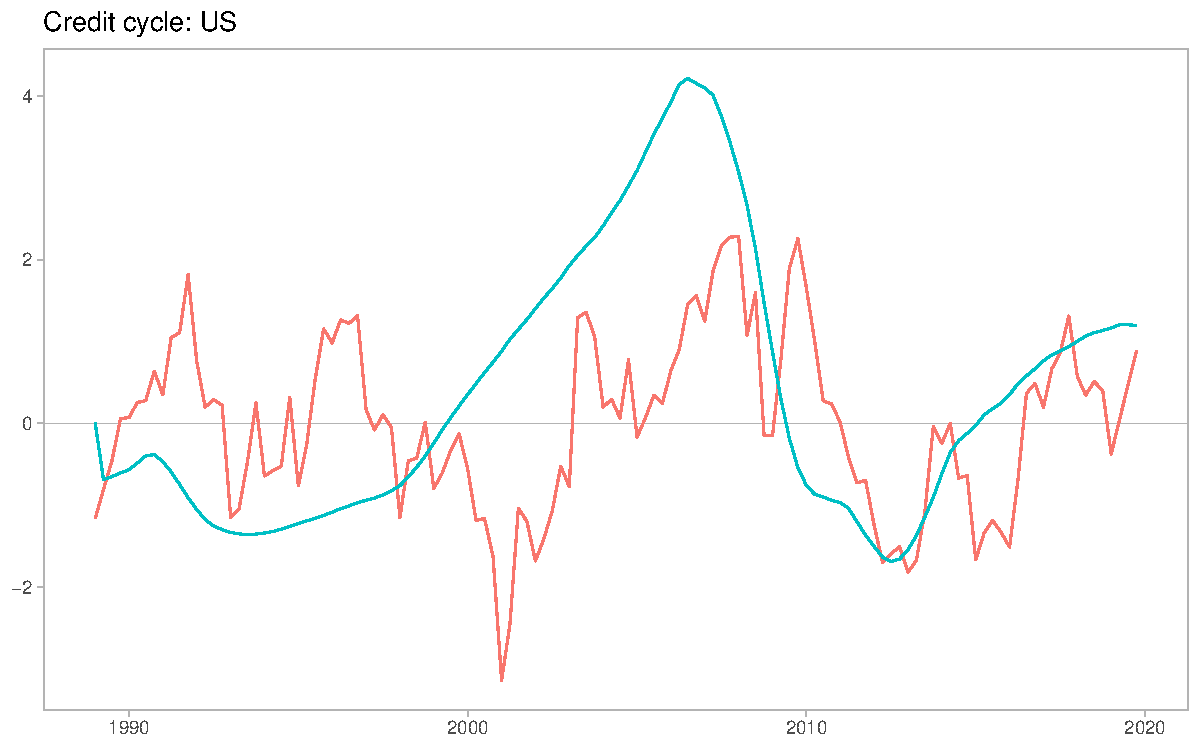
\includegraphics[scale=0.7]{../../Regression/VAR_2_crosscycle_1stlagonly/Output/Graphs/Credit_cycle_US.pdf}}
%			\centerline{\includegraphics[scale=0.7]{../../Regression/VAR_2_crosscycle_1stlagonly/Output/Graphs/HP_Cycle_US.pdf}}
%		\end{figure}
		
%		\begin{figure}[h!]
%			\caption{VAR(2) cross-cycle 1st lag US: Trend components}	
%			\centerline{\includegraphics[scale=0.7]{../../Regression/VAR_2_crosscycle_1stlagonly/Output/Graphs/Credit_trend_US.pdf}}
%			\centerline{\includegraphics[scale=0.7]{../../Regression/VAR_2_crosscycle_1stlagonly/Output/Graphs/HP_trend_US.pdf}}
%		\end{figure}
		
%		\begin{figure}[h!]
%			\caption{VAR(2) cross-cycle 1st lag UK: Cycle components}	
%			\centerline{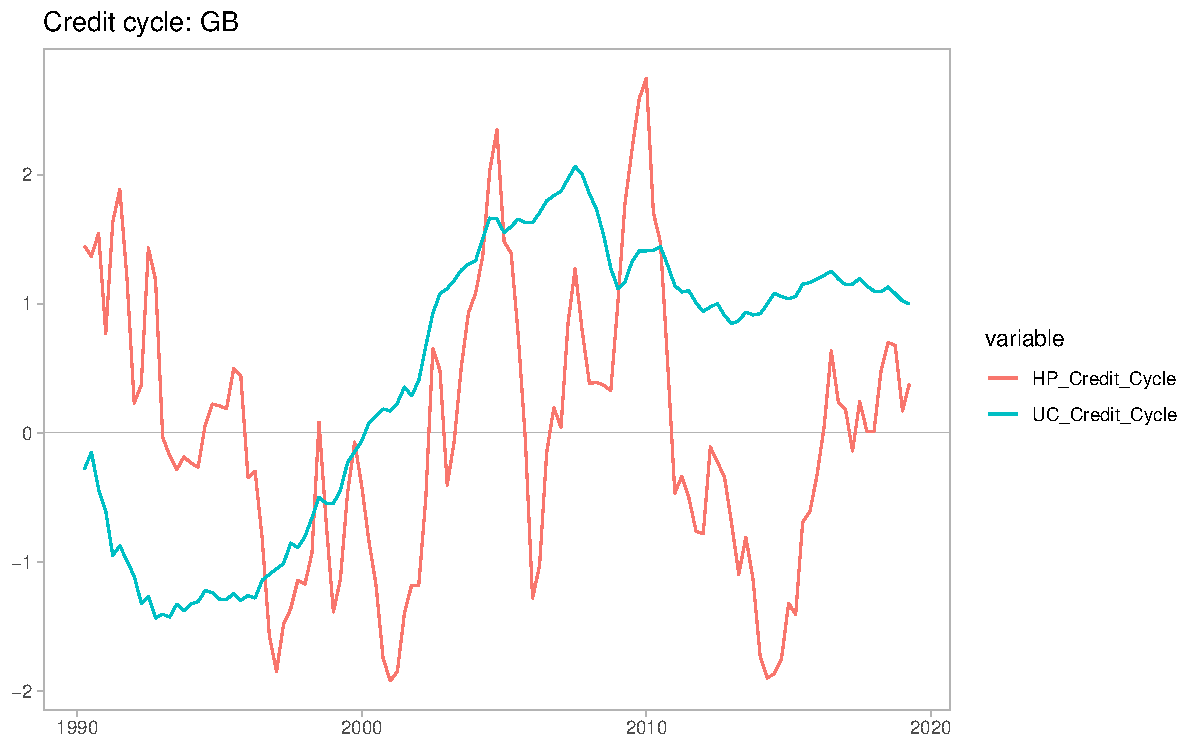
\includegraphics[scale=0.7]{../../Regression/VAR_2_crosscycle_1stlagonly/Output/Graphs/Credit_cycle_GB.pdf}}
%			\centerline{\includegraphics[scale=0.7]{../../Regression/VAR_2_crosscycle_1stlagonly/Output/Graphs/HP_Cycle_GB.pdf}}
%		\end{figure}
%		
%		\begin{figure}[h!]
%			\caption{VAR(2) cross-cycle 1st lag UK: Trend components}	
%			\centerline{\includegraphics[scale=0.7]{../../Regression/VAR_2_crosscycle_1stlagonly/Output/Graphs/Credit_trend_GB.pdf}}
%			\centerline{\includegraphics[scale=0.7]{../../Regression/VAR_2_crosscycle_1stlagonly/Output/Graphs/HP_trend_GB.pdf}}
%		\end{figure}
		
		\clearpage
		\section{Conclusion}
		Employing cross effects on the transitory components of the two series allows me to measure the effect of past short term shock from house hold credit on current housing price and vice versa.
				
		In this paper, the models for US and GB data shows that there is a positive relationship between a one period lag in short term house hold credit and current house price. 
		
		Further development for this paper should include more robust optimal constraints on parameters to ensure stability rather than an adhod approach to selecting. Additional examination of the multicolliearity / identification issue also needs to be addressed.
		
				
%		\section*{Appendix}
%
%		I will also include graphs that compare the 3 regression models forecast against HP filter cycle components.
		
		\clearpage
		
		
%		\begin{figure}[h!]
%			\caption{VAR(2) cross-cycle US: Cycle components}	
%			\centerline{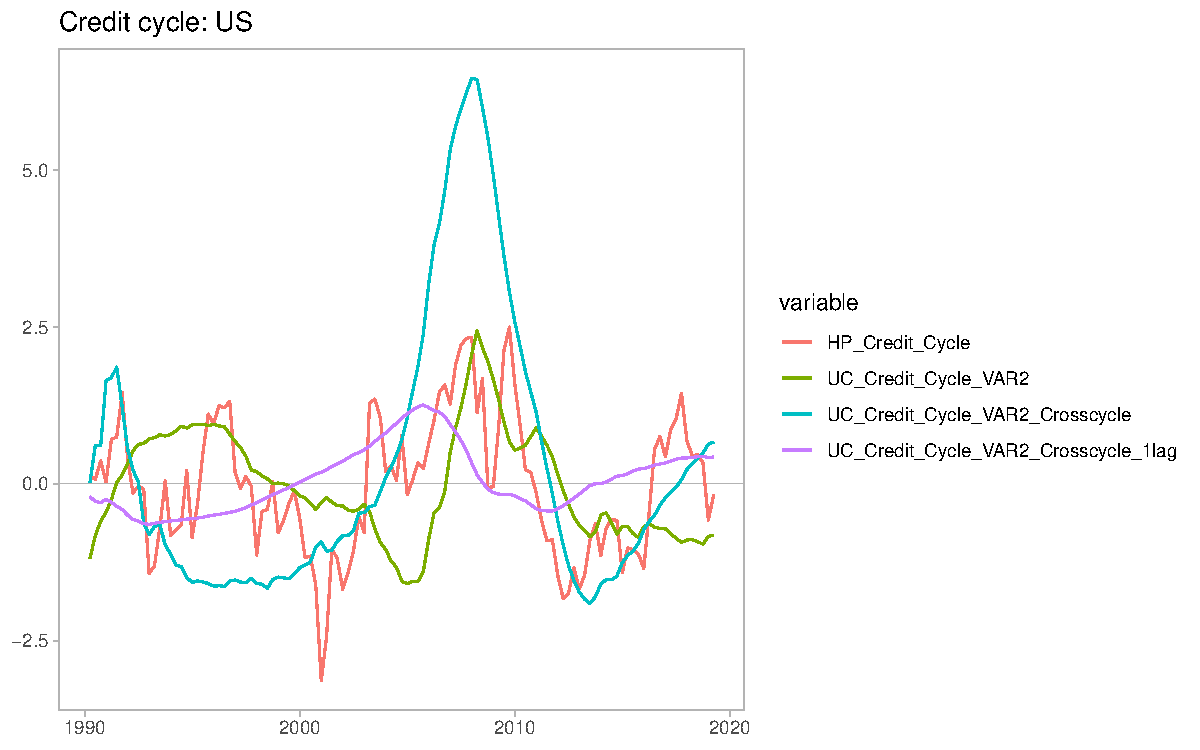
\includegraphics[scale=0.7]{../Graphs/Credit_cycle_US.pdf}}
%			\centerline{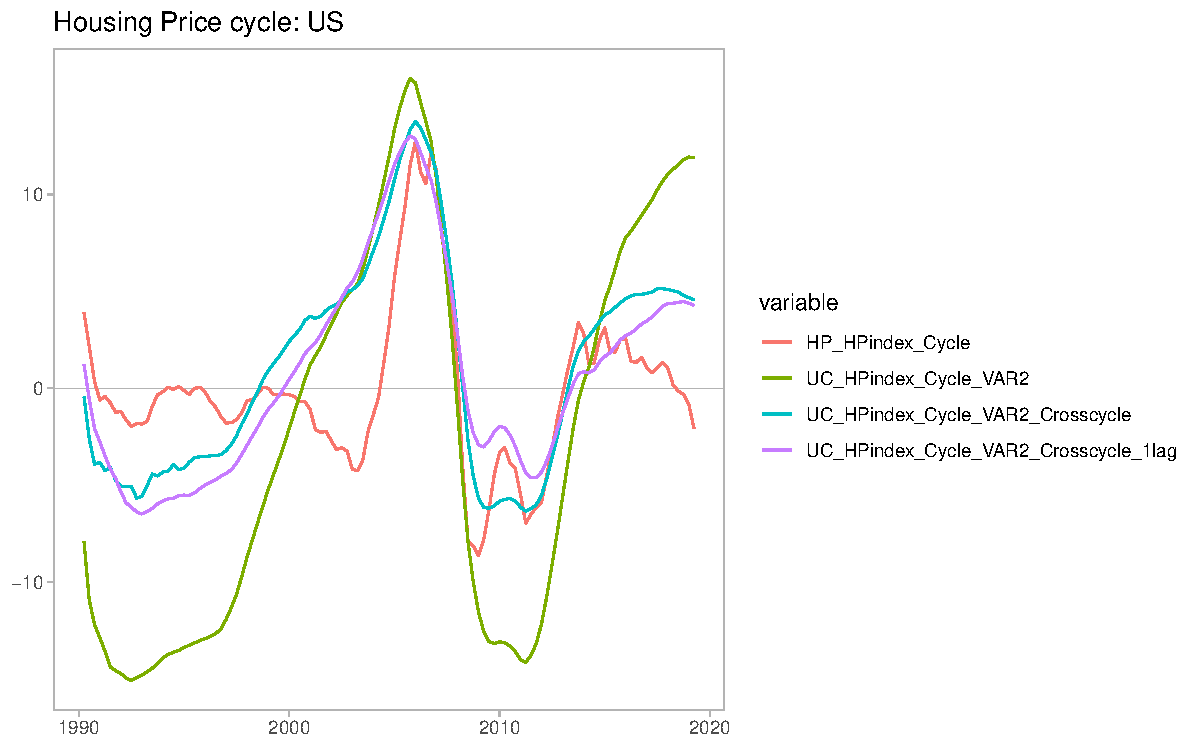
\includegraphics[scale=0.7]{../Graphs/HP_cycle_US.pdf}}
%		\end{figure}
		

		
		%
		%\begin{figure}[h!]
		%	\caption{Germany Credit components}	
		%	\centerline{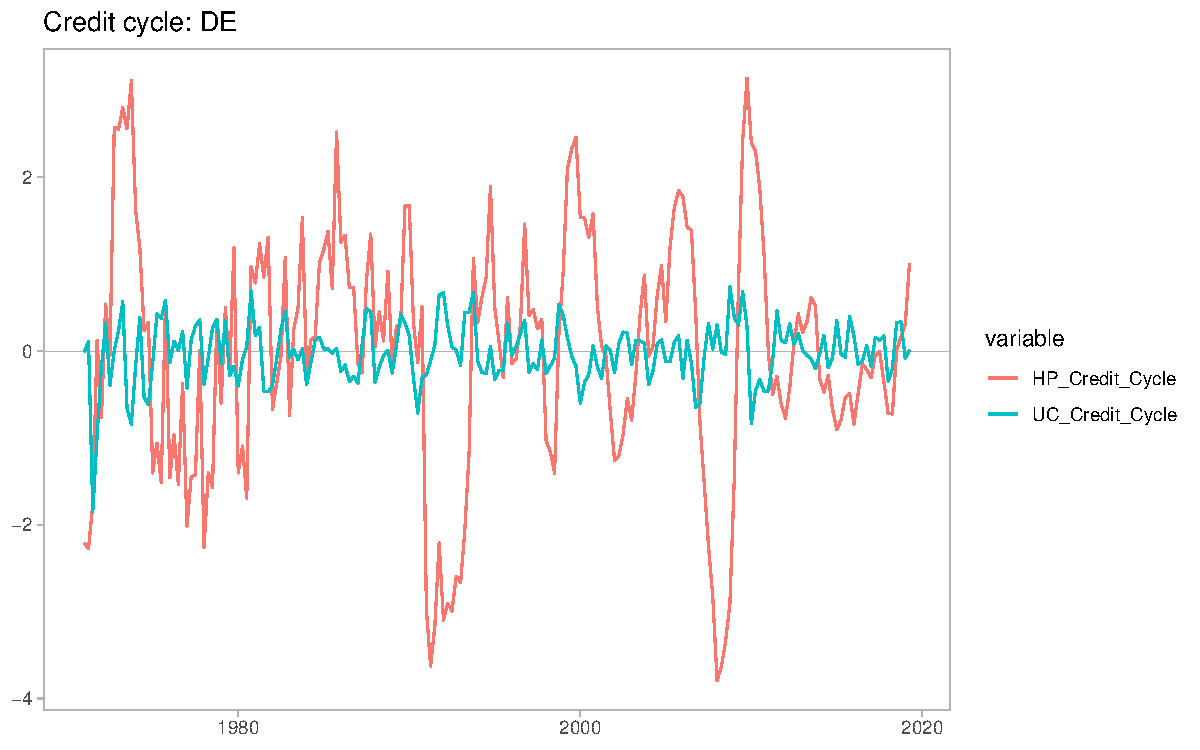
\includegraphics[scale=0.7]{../Output/Graphs/Credit_cycle_DE.pdf}}
		%	\centerline{\includegraphics[scale=0.7]{../Output/Graphs/Credit_trend_DE.pdf}}
		%\end{figure}
		%
		%\begin{figure}[h!]
		%	\caption{Germany Housing Price components}	
		%	\centerline{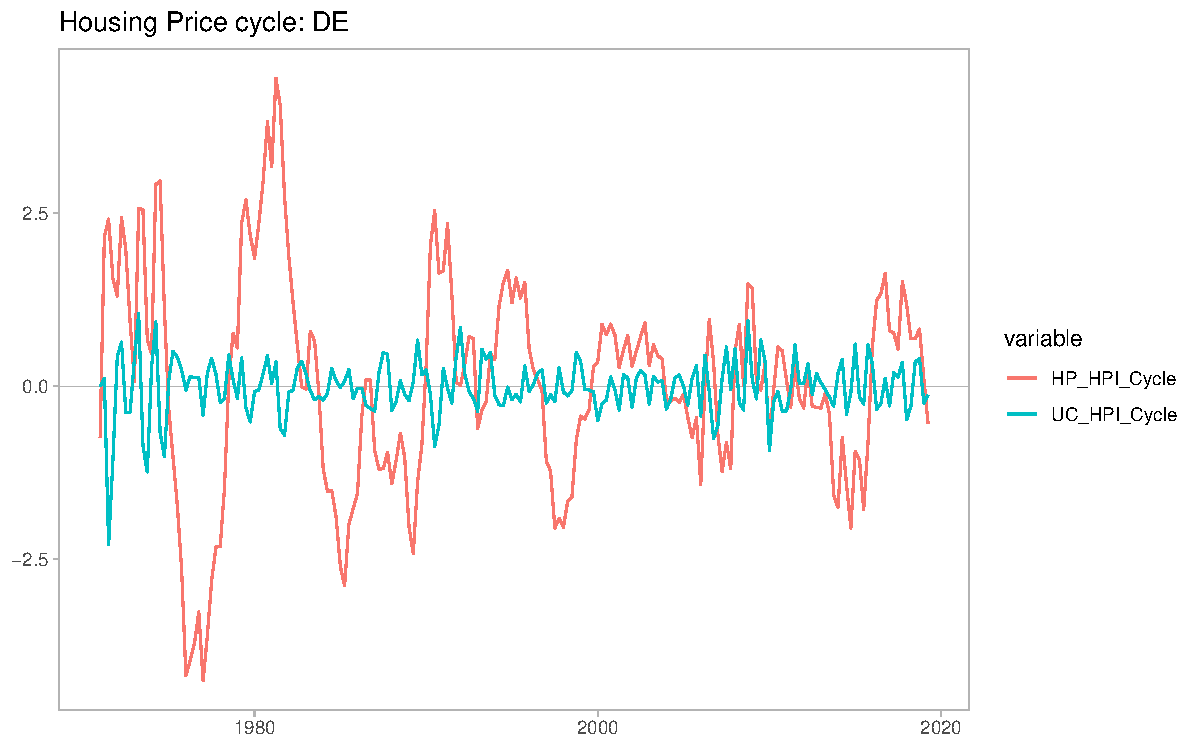
\includegraphics[scale=0.7]{../Output/Graphs/HP_cycle_DE.pdf}}
		%	\centerline{\includegraphics[scale=0.7]{../Output/Graphs/HP_trend_DE.pdf}}
		%\end{figure}
		%
		%
		%\begin{figure}[h!]
		%	\caption{France Credit components}	
		%	\centerline{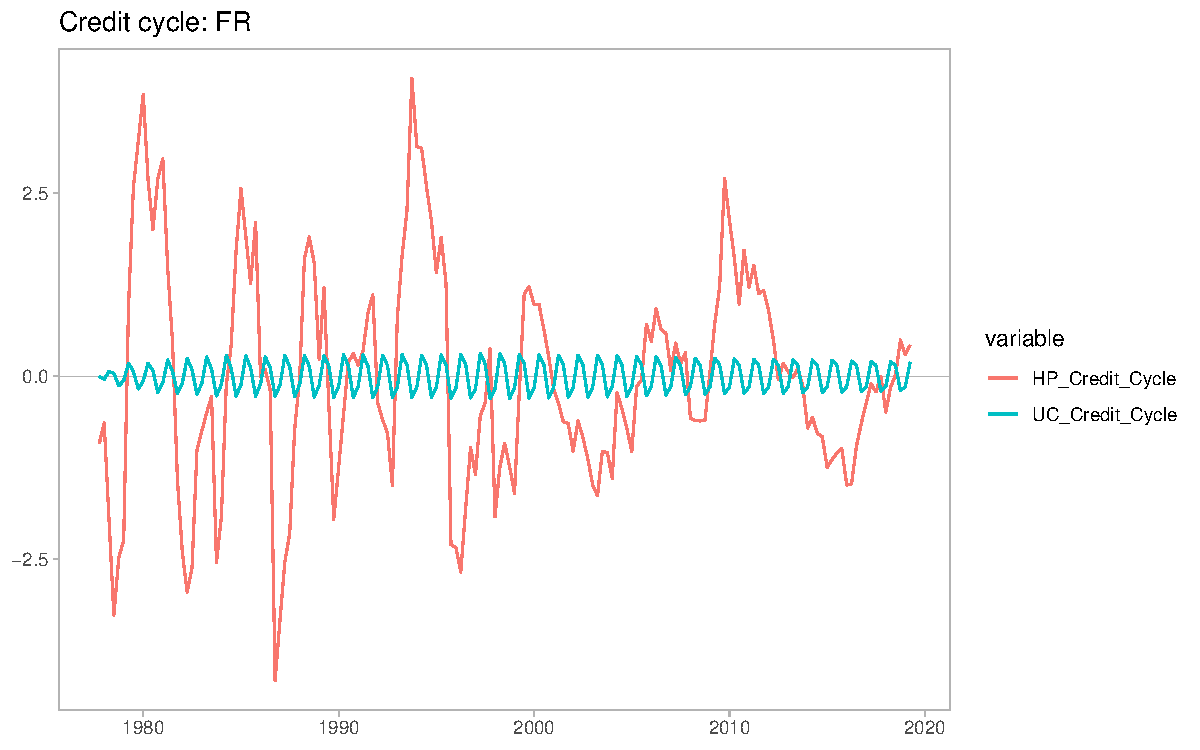
\includegraphics[scale=0.7]{../Output/Graphs/Credit_cycle_FR.pdf}}
		%	\centerline{\includegraphics[scale=0.7]{../Output/Graphs/Credit_trend_FR.pdf}}
		%\end{figure}
		%
		%\begin{figure}[h!]
		%	\caption{France Housing Price components}	
		%	\centerline{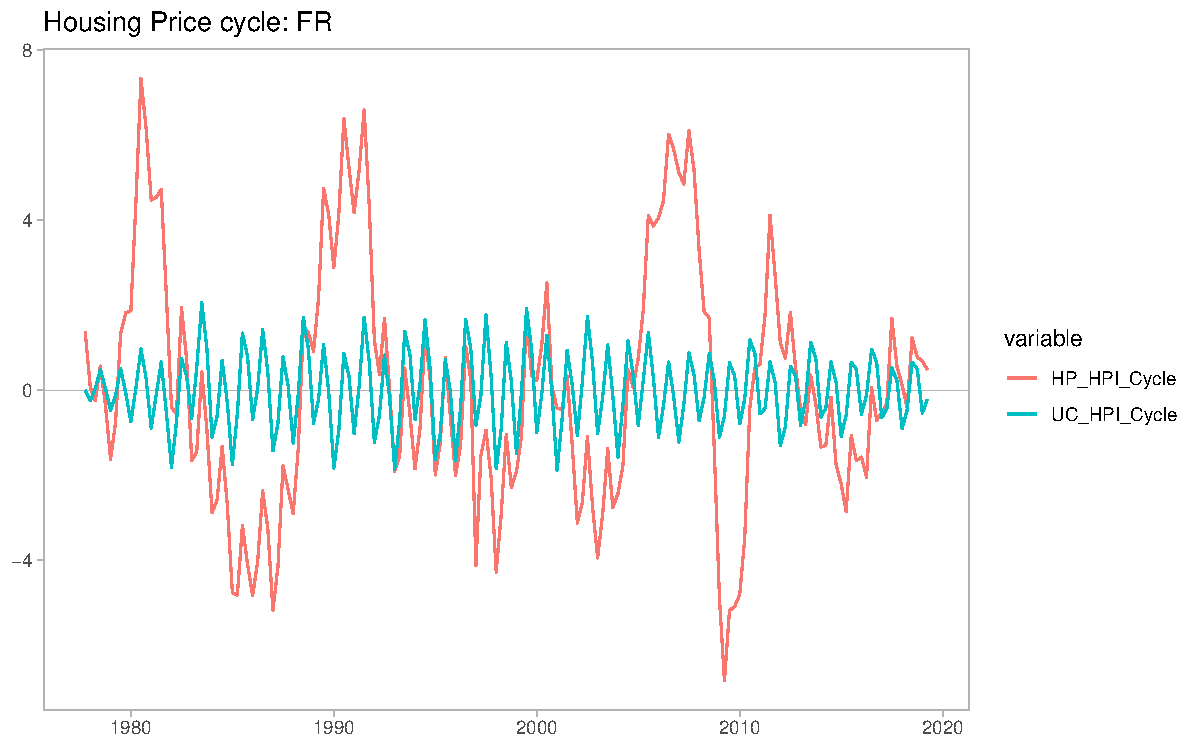
\includegraphics[scale=0.7]{../Output/Graphs/HP_cycle_FR.pdf}}
		%	\centerline{\includegraphics[scale=0.7]{../Output/Graphs/HP_trend_FR.pdf}}
		%\end{figure}
		%
		%
		%\begin{figure}[h!]
		%	\caption{Japan Credit components}	
		%	\centerline{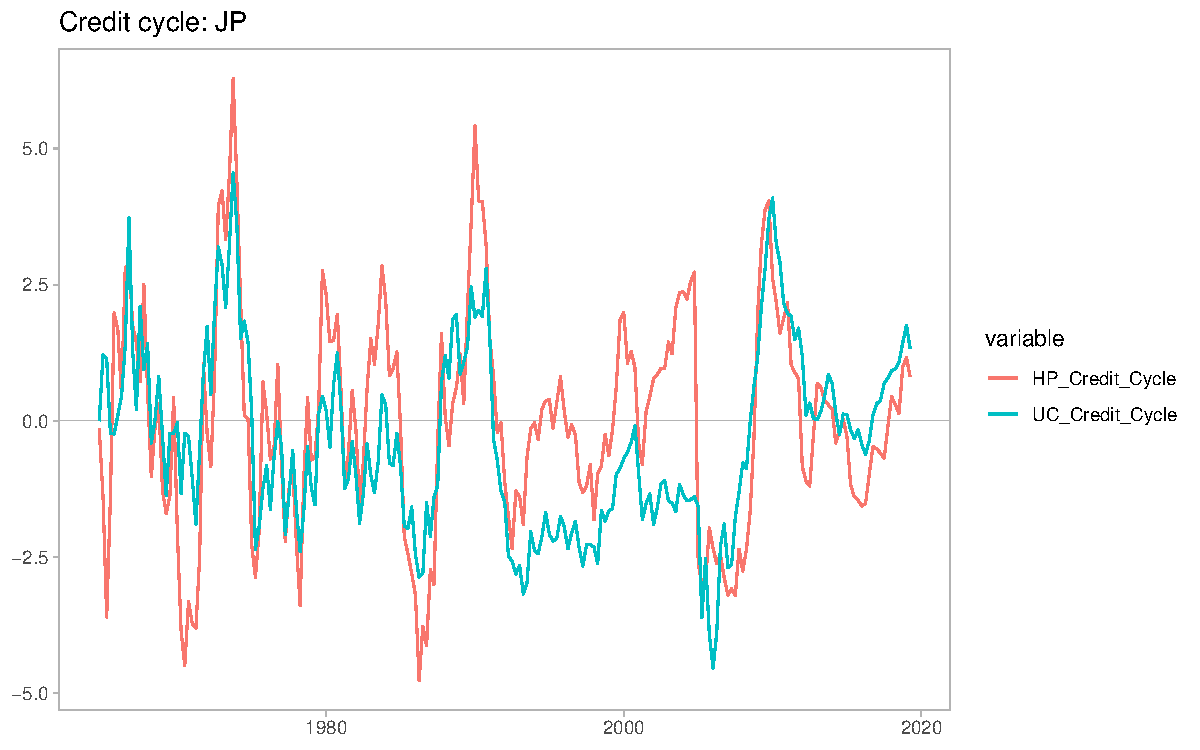
\includegraphics[scale=0.7]{../Output/Graphs/Credit_cycle_JP.pdf}}
		%	\centerline{\includegraphics[scale=0.7]{../Output/Graphs/Credit_trend_JP.pdf}}
		%\end{figure}
		%
		%\begin{figure}[h!]
		%	\caption{Japan Housing Price components}	
		%	\centerline{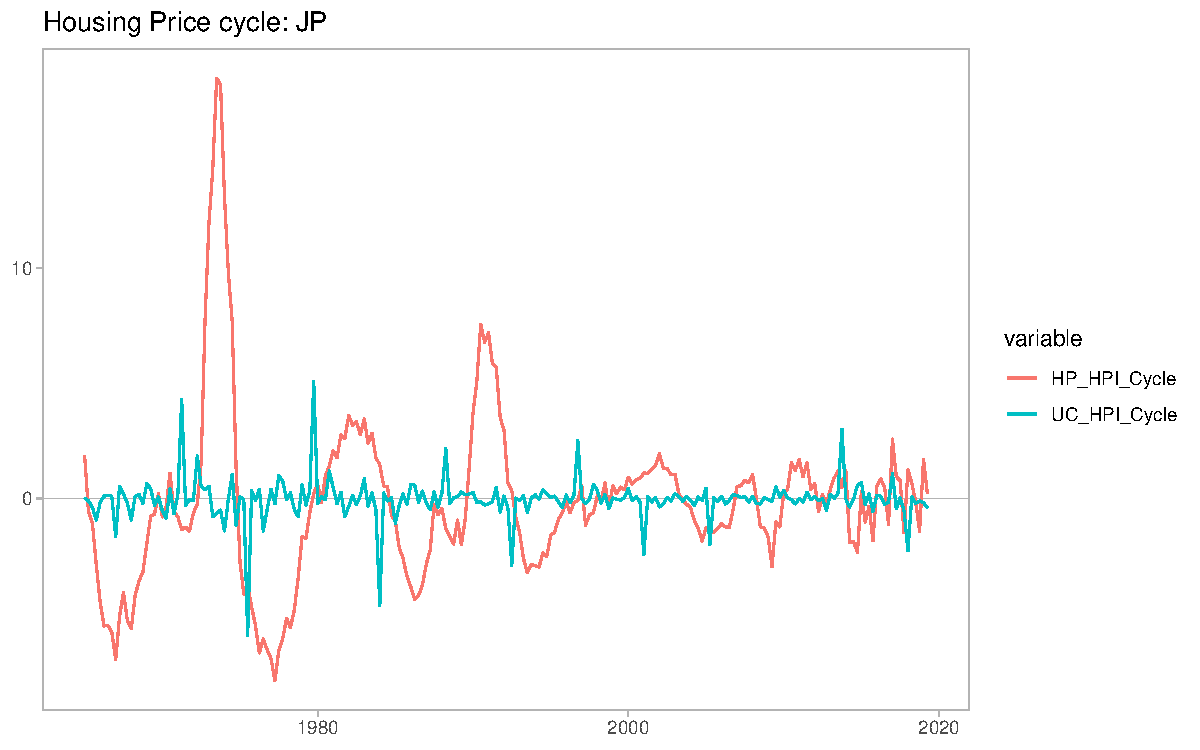
\includegraphics[scale=0.7]{../Output/Graphs/HP_cycle_JP.pdf}}
		%	\centerline{\includegraphics[scale=0.7]{../Output/Graphs/HP_trend_JP.pdf}}
		%\end{figure}
		%
		%
		%\begin{figure}[h!]
		%	\caption{Korea Credit components}	
		%	\centerline{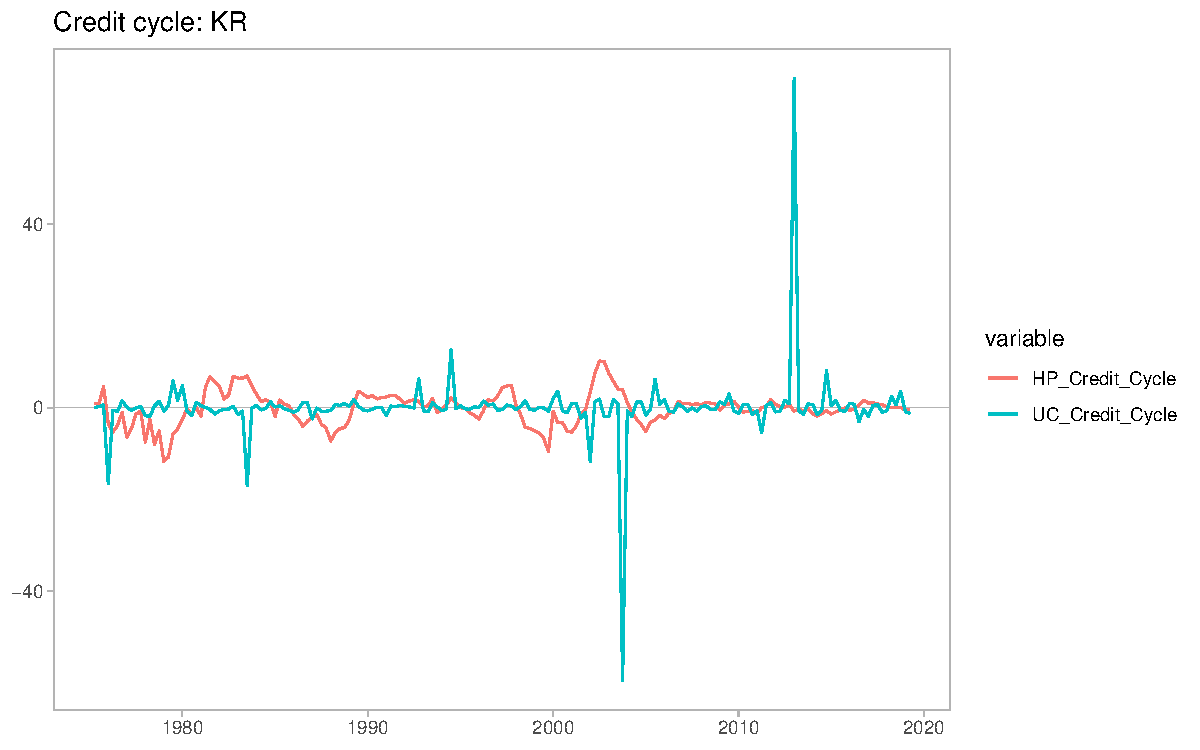
\includegraphics[scale=0.7]{../Output/Graphs/Credit_cycle_KR.pdf}}
		%	\centerline{\includegraphics[scale=0.7]{../Output/Graphs/Credit_trend_KR.pdf}}
		%\end{figure}
		%
		%\begin{figure}[h!]
		%	\caption{Korea Housing Price components}	
		%	\centerline{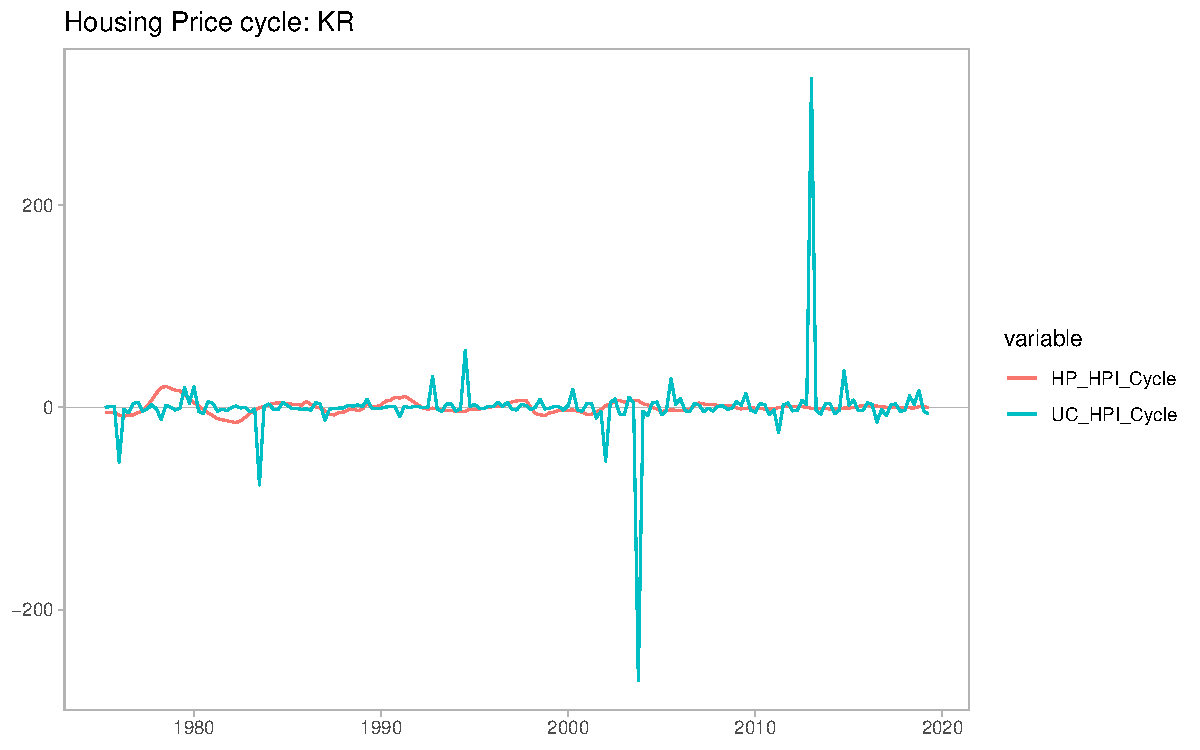
\includegraphics[scale=0.7]{../Output/Graphs/HP_cycle_KR.pdf}}
		%	\centerline{\includegraphics[scale=0.7]{../Output/Graphs/HP_trend_KR.pdf}}
		%\end{figure}
		
		\clearpage
		%
		%\section{Impulse Response Function}
		%
		%
		%
		%This section show IRFs that are really unstable. I am guessing that is because the way I specify the function:
		%
		%Instead of normally having: $\psi_t = \phi^y_{11}*\psi_l + \phi^y_{12}*\psi_{ll}$
		%
		%I specify the IRF as: $\psi_t = \phi^y_{11}*\psi_l + \phi^y_{12}*\psi_{ll} + \phi^y_{21}*\psi_l + \phi^y_{22}*\psi_{ll} $
		%\\
		%This potentially causes the unstability in the following IRF graphs. Also the fact that the constraints for autoregressive parameters have not been optimally setup could cause the issue.
		%
		%
		%\begin{figure}[h!]
		%	\caption{US IRF}	
		%	\centerline{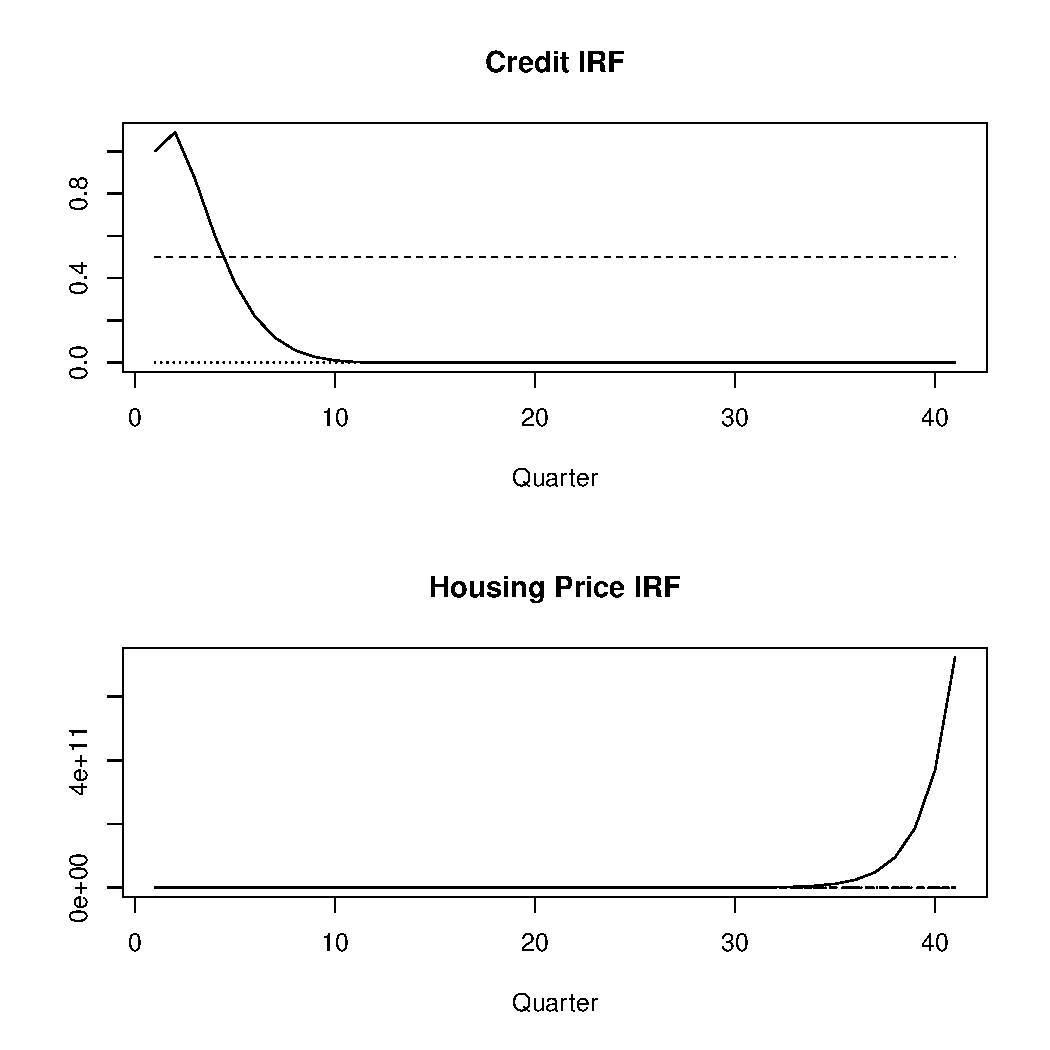
\includegraphics[scale=0.7]{../Output/Graphs/IRF_US.pdf}}
		%\end{figure}
		%
		%\begin{figure}[h!]
		%	\caption{UK IRF}	
		%	\centerline{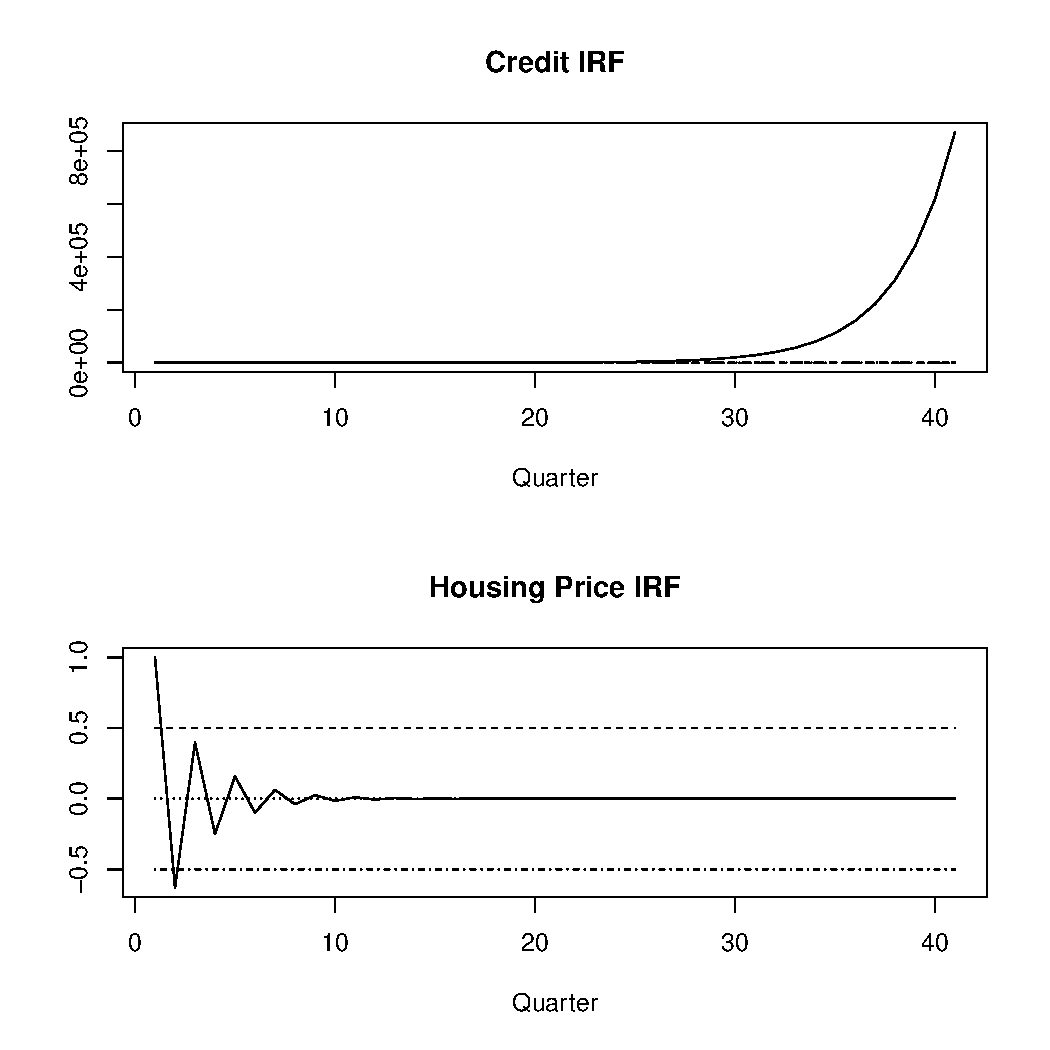
\includegraphics[scale=0.7]{../Output/Graphs/IRF_GB.pdf}}
		%\end{figure}
		%
		%\begin{figure}[h!]
		%	\caption{Germany IRF}	
		%	\centerline{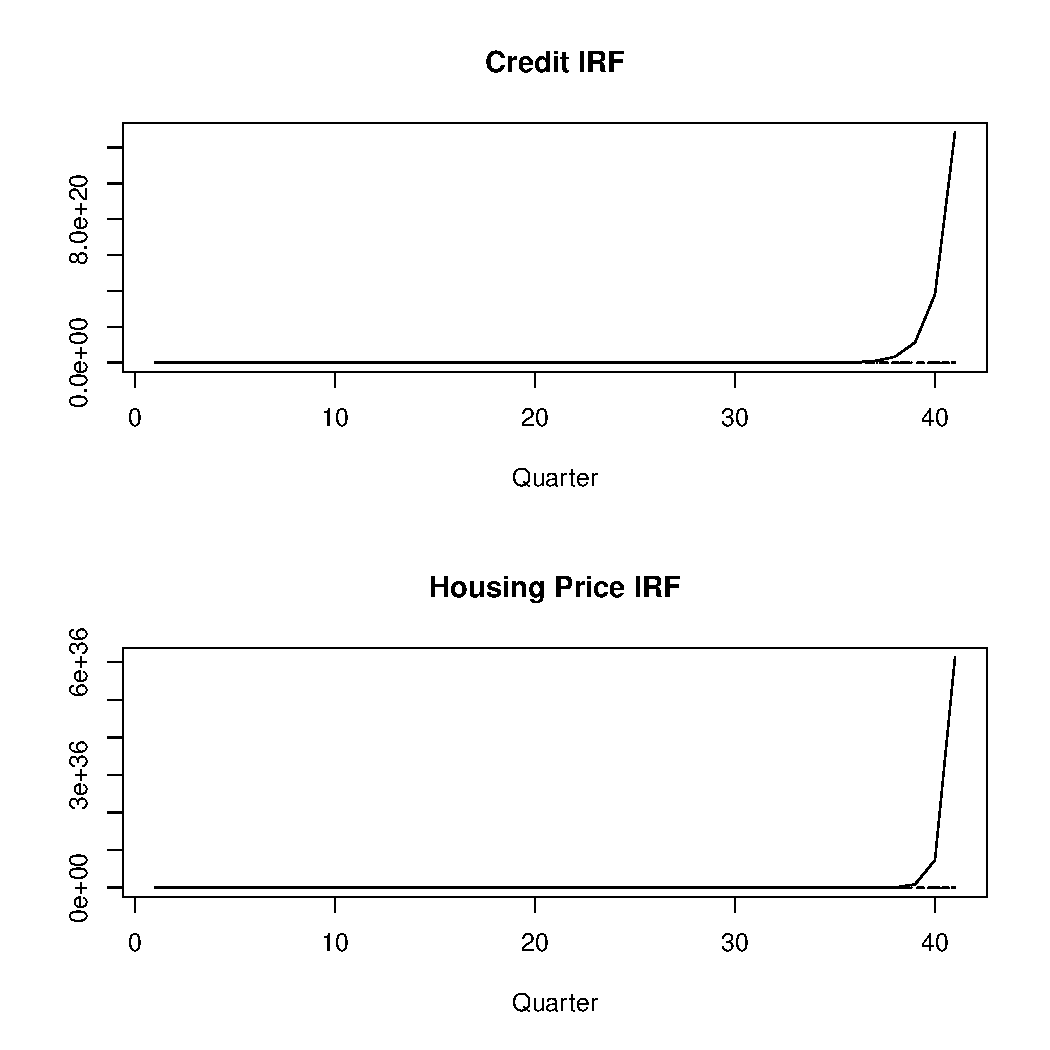
\includegraphics[scale=0.7]{../Output/Graphs/IRF_DE.pdf}}
		%\end{figure}
		%
		%\begin{figure}[h!]
		%	\caption{France IRF}	
		%	\centerline{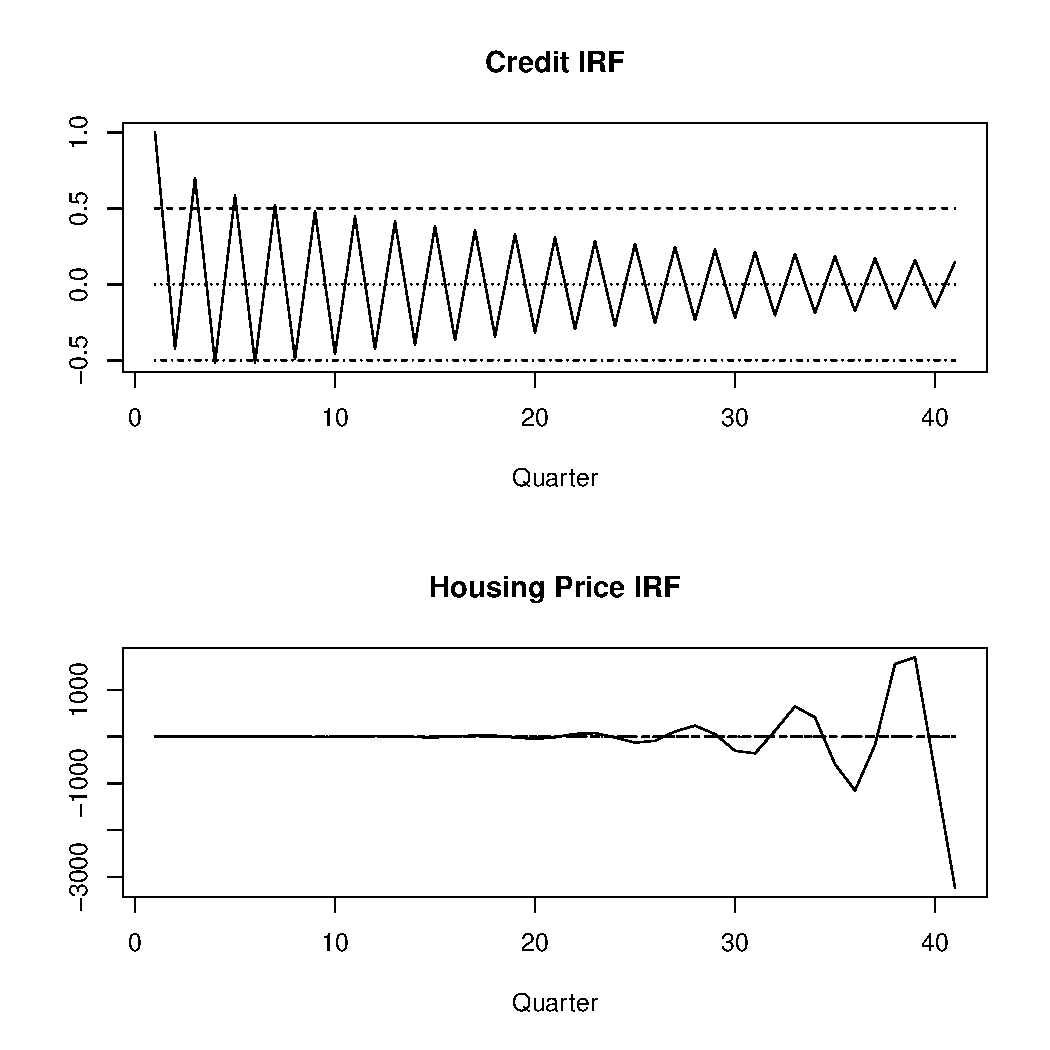
\includegraphics[scale=0.7]{../Output/Graphs/IRF_FR.pdf}}
		%\end{figure}
		%
		%\begin{figure}[h!]
		%	\caption{Japan IRF}	
		%	\centerline{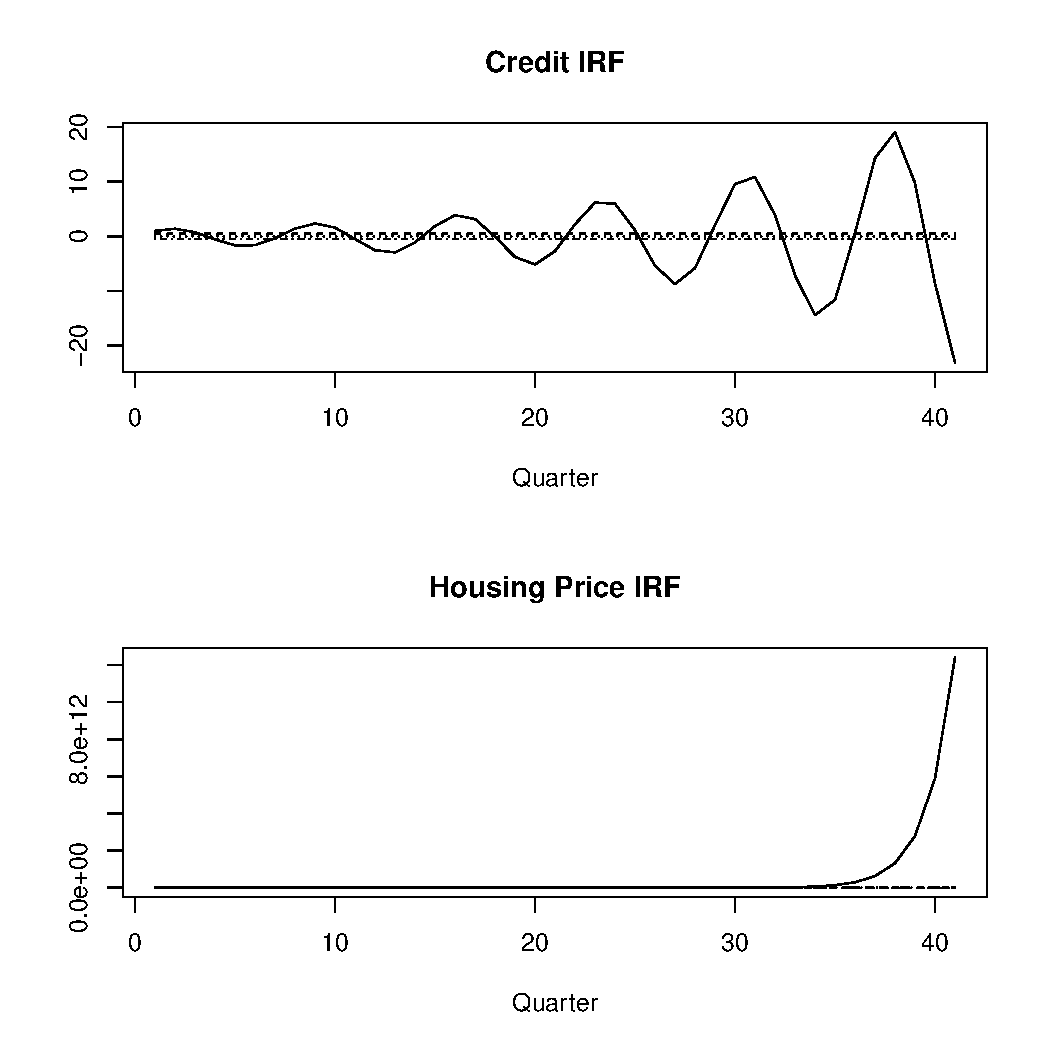
\includegraphics[scale=0.7]{../Output/Graphs/IRF_JP.pdf}}
		%\end{figure}
		%
		%\begin{figure}[h!]
		%	\caption{Korea IRF}	
		%	\centerline{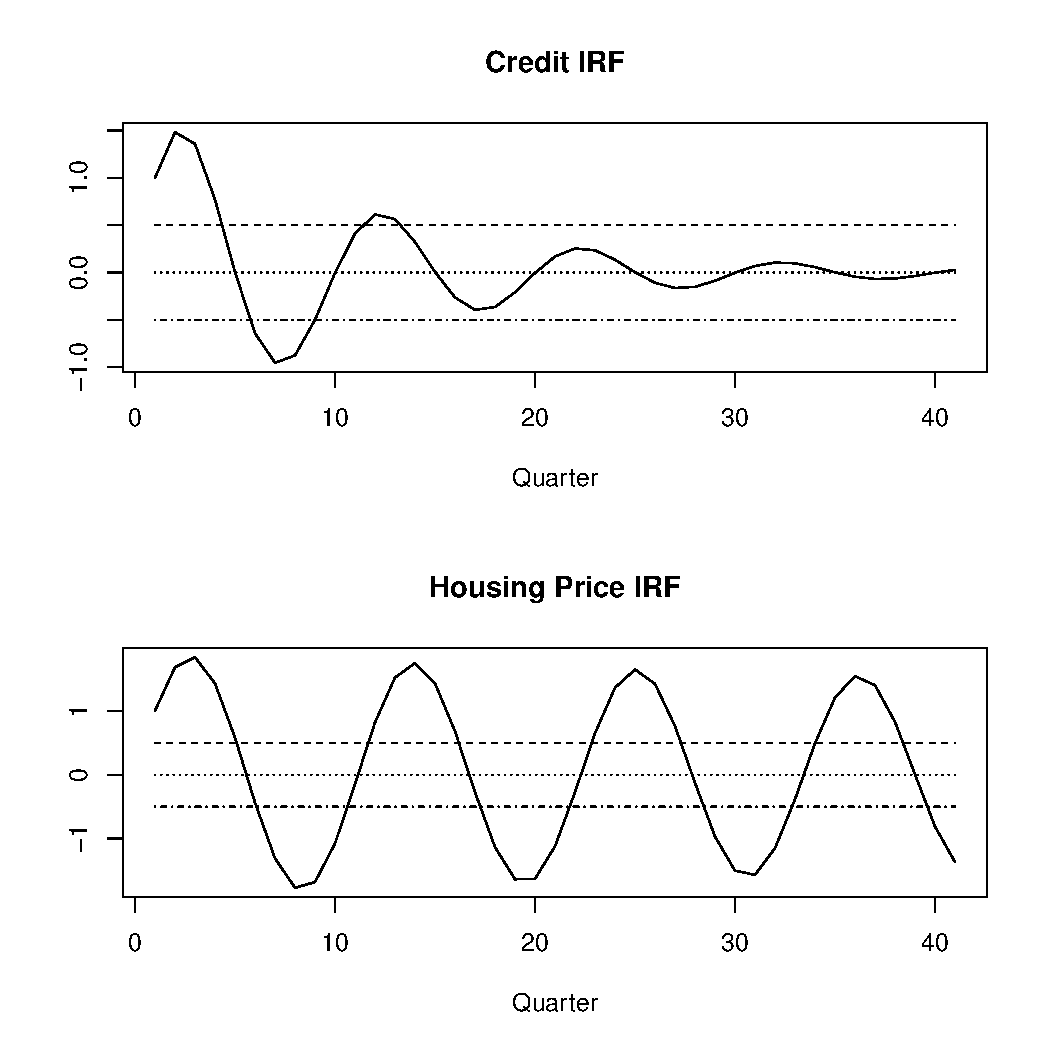
\includegraphics[scale=0.7]{../Output/Graphs/IRF_KR.pdf}}
		%\end{figure}
		
		
		
		
	\end{outline}
\end{document}